\documentclass[11pt]{article}
\usepackage[margin=1in]{geometry}
\usepackage{amsmath,amssymb}
\usepackage{graphicx}
\usepackage{tikz}
\usepackage[numbers]{natbib}
\usepackage{hyperref}

\title{A Short Note on Damped Oscillators}
\author{Demo Author}
\date{\today}

\begin{document}
\maketitle

\begin{abstract}
We revisit the damped harmonic oscillator and derive its three regimes.
This short note is a demo project for texc.
It has an abstract, sections in separate files, equations, a figure and citations.
\end{abstract}

\section{Introduction}\label{sec:intro}
Oscillators are everywhere, from pendulum clocks to MEMS resonators.
Section~\ref{sec:model} states the model and Section~\ref{sec:regimes} classifies its solutions.


\section{Model}\label{sec:model}
The displacement $x(t)$ of a mass $m$ on a spring with stiffness $k$ and damping $c$ obeys
\begin{equation}\label{eq:ode}
  m\ddot{x} + c\dot{x} + kx = 0 .
\end{equation}
With $\omega_0 = \sqrt{k/m}$ and $\zeta = c / (2\sqrt{mk})$, Eq.~\eqref{eq:ode} becomes
\begin{equation}
  \ddot{x} + 2\zeta\omega_0\dot{x} + \omega_0^2 x = 0 .
\end{equation}

\section{Regimes}\label{sec:regimes}
The roots of the characteristic polynomial are $\lambda = -\zeta\omega_0 \pm \omega_0\sqrt{\zeta^2-1}$.
The system is underdamped for $\zeta<1$, critically damped for $\zeta=1$ and overdamped for $\zeta>1$ \citep{goldstein2002}.
Figure~\ref{fig:decay} sketches the underdamped case.

\begin{figure}[h]
  \centering
  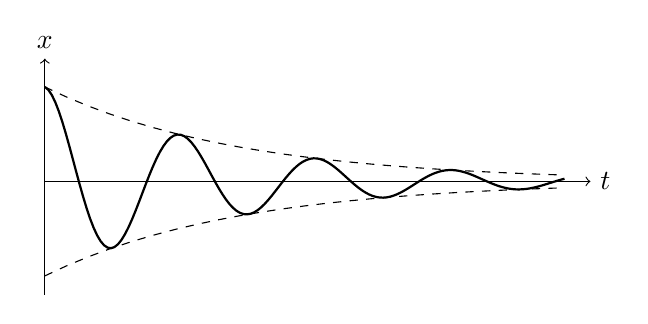
\begin{tikzpicture}[xscale=1.1,yscale=1.2]
    \draw[->] (0,0) -- (6.3,0) node[right] {$t$};
    \draw[->] (0,-1.2) -- (0,1.3) node[above] {$x$};
    \draw[thick,domain=0:6,samples=150] plot (\x,{exp(-0.45*\x)*cos(4*\x r)});
    \draw[dashed,domain=0:6] plot (\x,{exp(-0.45*\x)});
    \draw[dashed,domain=0:6] plot (\x,{-exp(-0.45*\x)});
  \end{tikzpicture}
  \caption{Underdamped response with its exponential envelope.}
  \label{fig:decay}
\end{figure}

\section{Conclusion}
Damping sets the regime; see \citet{strogatz2015} for the nonlinear story.

\bibliographystyle{plainnat}
\bibliography{refs}
\end{document}
